% !TEX root = ../../../../report.tex

\subsubsection{Power Supply}

The power supply is a big part of the PCB design, consisting of several
components. Being the energy efficiency group, maximizing power utilization
along with minimizing energy consumption has been of high priority, to make sure
as little power as possible goes to waste. When deciding on a design, the work
of previous groups was examined, particularly that of the energy efficiency
group of 2012. Anything before 2012 had more or less used the same power supply
used the same power supply, which was designed to transform any excess power
into heat. This is a simple and effective design, but not very efficient in
terms of power saving as it utilizes only a fraction of the input power.

Fortunately, the energy efficiency group of 2012 did a solid job on their power
supply, using a switch-mode regulator that is able to output 3.3V from any input
voltage ranging from 4.75V up to 18V with an efficiency of 83-90\%~\cite{ds:sr10s3v3}. This is very efficient, so most of the design
was copied except for a change in current sensors, which is explained in detail
below.

\begin{figure}[H]
    \centering
    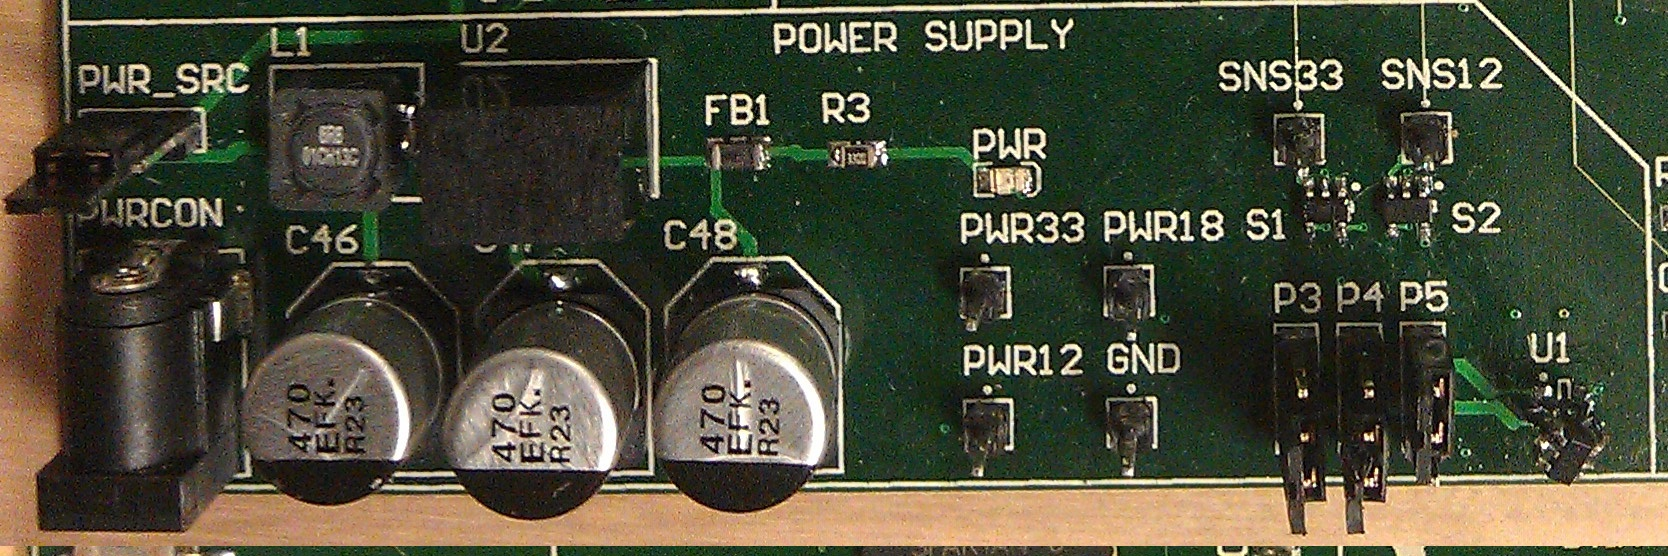
\includegraphics[scale=0.15]{figures/intro/pcb/bitless_psu}
    \caption{The power supply}
    \label{fig:psu}
\end{figure}


\paragraph{Voltage Regulators}

The design is based on a switch-mode regulator that transforms DC input into
3.3V~\cite{ds:sr10s3v3}, and a linear regulator \cite{ds:linreg}
that transforms 3.3V into 1.2V and 1.8V, see power\_supply schematics in Appendix~\ref{apx:schematics}. The switch-mode gets an input voltage between 4.75V
and 18V which, as mentioned, is transformed into 3.3V and kept stable by
capacitors. This in turn supplies the 3.3V input for the linear voltage
regulator that delivers both the 1.2V and the 1.8V output. Originally it was
intended to disable the 1.8V domain entirely, running the whole board on 1.2V
and 3.3V, but as the FPGA was changed midway to a slightly larger one, the FPGA
flash also had to be changed and the new one required 1.8V.

The design efficiently delivers power at these three voltages. Very
little power goes to waste in the switch-mode regulator, and while the linear
regulator transforms power into heat, transforming from 3.3V instead of, for
example 9V, is a large improvement.

\paragraph{Current Sensors} \label{psu:current_sensors}

The main problem with the 2012 design was that the current sensors were not
sensitive enough for low voltages, which resulted in inaccurate measurements. To
remedy this the current sensors were changed to more fitting ones. One has been
placed on the 3.3V power plane, while the other sits just before the linear
regulator. This way, it is possible to separate the 3.3V plane from the 1.2V and
1.8V, which enables analysis of MCU and FPGA power consumption in comparison
with the peripherals. In addition, the entire board consumption can be measured
at the PWR\_SRC pins located right after the DC input connector, see power\_supply schematics in Appendix~\ref{apx:schematics} and measurements in Section \ref{power_measurements}.

The output from the current sensors have each been connected to an ADC on the
MCU, which makes it possible to perform live measurements on-chip. However, by
performing measurements using the MCU, the results are skewed, as reading the
ADC increases power consumption. Therefore, measuring sockets have been added to
allow for reading the current sensor output on an external device, such as a
development board, making for more accurate readings.

\paragraph{Power by USB} \label{psu:usb}

An extra feature that was added was the ability to power the board from USB. The
USB 1.x and 2.0 standard specifies that a constant power draw of 500mA at 5.0V
$\pm$ 5\% can be provided \cite{usb}. This should suffice for
normal operation. USB chargers will in most cases provide support for current
draws in the 1500mA to 2000mA range, so using one of these should be able to
supply sufficient power through the USB port.

Even when using the normal power socket as the primary power supply, parts of
the board will still be powered through USB. This includes the UART-USB bridge
and the related TX and RX LEDs. By powering these components with power from the
USB, all parts related to the USB connectivity will be completely powered down
when no USB cable is connected.
